\section{Um problema prático}

Para testar as características de AGs discutidas anteriormente, optou-se por implementar o AG descrito por \textcite{SEDIGHI2004}. Trata-se de um método para determinar a rota que um robô móvel deve seguir em um mapa de modo a concluir um trajeto que minimize a distância percorrida, o número de curvas e o número de colisões contra obstáculos. Para implementar este AG e testar seus resultados, utilizou-se a linguagem de programação Julia \cite{BEZANSON2015}. As seções seguintes são dedicadas a explicar as etapas do AG implementado, bem como as escolhas feitas durante a implementação do código, que pode ser encontrado em \href{https://github.com/phcentenaro7/GA-Robotica}{repositório virtual}.

\subsection{Componentes do mapa}

Assume-se que o robô tenha o mapa completo do ambiente, visto de cima, antes de iniciar o AG, e que os obstáculos sejam retangulares. Para que a roteirização possa ser implementada, é necessário discretizar o mapa, de modo que existam pontos bem-definidos pelos quais o robô possa passar. De fato, o próprio robô é considerado pontual neste sistema.

Para definir um mapa, inicia-se definindo os obstáculos presentes. Isso é feito por meio da função \texttt{obstaculo}, que recebe as coordenadas e as dimensões do objeto no plano. Após criar uma lista de obstáculos, é necessário fazer a discretização do mapa por meio da função \texttt{criar\_ecra}. Esta função recebe a lista de obstáculos e a largura do mapa -- como é explicado adiante, este AG depende de mapas quadrados para funcionar; portanto, caso um mapa não seja quadrado, é necessário distorcê-lo de acordo com o necessário. Um parâmetro adicional de \emph{tamanho de passo}, $\Delta$, pode ser especificado. Trata-se da distância entre dois pontos da discretização, que, por padrão, é 1. O que a função \texttt{criar\_ecra} retorna é uma matriz \emph{booleana} quadrada especificando quais pontos discretizados correspondem a espaços livres no mapa, e quais correspondem a espaços ocupados por obstáculos.

Para visualizar o mapa criado, basta chamar a função \texttt{mapear}, que recebe a lista de obstáculos e a largura do mapa como argumentos. Opcionalmente, é possível passar a matriz de ecrã para esta função, junto com o tamanho de passo, para mostrar o resultado da discretização do mapa. A \cref{fig:mapa exemplo 1} mostra o exemplo de um mapa e sua discretização. As partes brancas do mapa são locais pelos quais o robô pode passar; as partes pretas são obstáculos. Os pontos representam a discretização do mapa, sendo azuis os pontos pelos quais o robô pode passar e vermelhos os pontos indicativos de colisão. O \cref{cod:código mapa} foi usado para gerar este mapa.

\begin{figure}[ht]
    \centering
    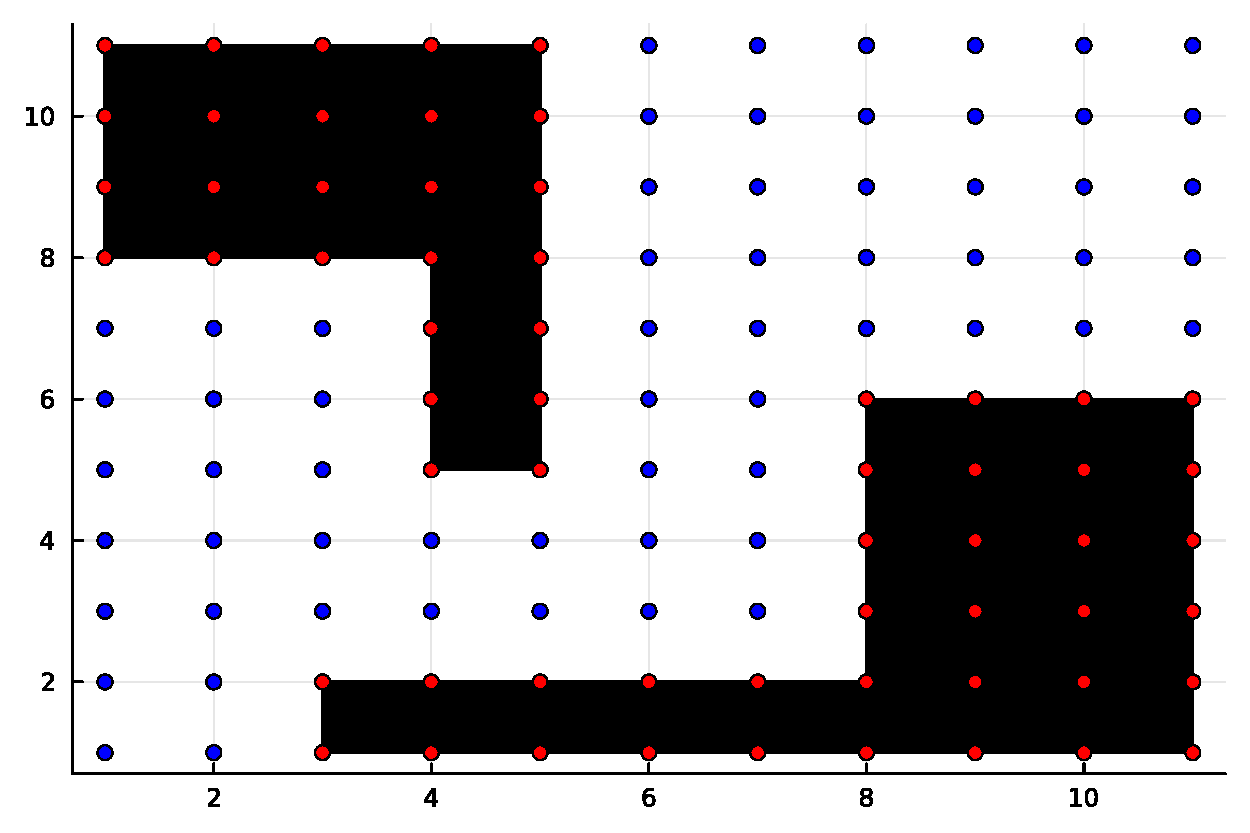
\includegraphics[scale=0.6]{images/exemplo_mapa.pdf}
    \caption{Exemplo de mapa discretizado.}
    \label{fig:mapa exemplo 1}
\end{figure}

\begin{figure}[ht]
    \centering
    \begin{minted}{julia}
        obs = [obstaculo(1, 4, 8, 3),
        obstaculo(4, 1, 5, 3),
        obstaculo(3, 7, 1, 1),
        obstaculo(8, 3, 1, 5)]
        largura = 10
        ∆ = 1
        E = criar_ecra(obs, largura, Δ=Δ)
        grafico = mapear(obs, largura, ecra=E, Δ=Δ)
    \end{minted}
    \renewcommand{\figurename}{Código}
    \caption{Código para geração de mapa.}
    \label[code]{cod:código mapa}
\end{figure}

\subsection{Cromossomos e funções de aptidão}

Os cromossomos propostos por \textcite{SEDIGHI2004} são divididos em quatro segmentos, como ilustra a \cref{fig:cromossomo roteirização}. O primeiro alelo contém um gene binário chamado \emph{path} (caminho). O papel deste gene é indicar se o robô realizará deslocamentos \emph{row-wise} ou \emph{column-wise}. Estes movimentos só podem ser entendidos com a descrição da seção \emph{location} (localização), que consiste em $n$ alelos que descrevem uma sequência de pontos discretizados pelos quais o robô deve passar.

\begin{figure}[ht]
    \centering
    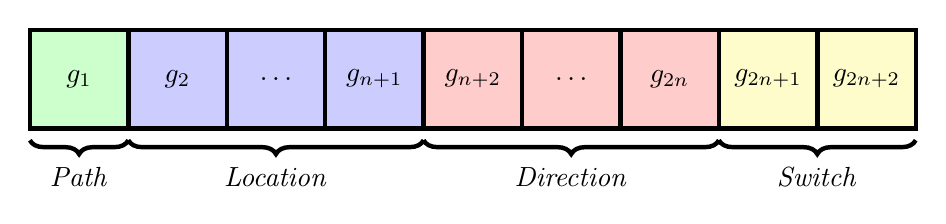
\begin{tikzpicture}
        \foreach \x/\y/\color in {1/g_1/green!20,2/g_2/blue!20,3/\dots/blue!20,4/g_{n+1}/blue!20,5/g_{n+2}/red!20,6/\dots/red!20,7/g_{2n}/red!20,8/g_{2n+1}/yellow!20,9/g_{2n+2}/yellow!20}
        {
            \draw[fill=\color, ultra thick] (1.25*\x, 0) rectangle ++(1.25, 1.25) node[pos=.5] {$\y$};
        }
        \draw[decorate,decoration={brace,amplitude=5pt,mirror,raise=1ex},ultra thick] (1.25, 0) -- (2.5, 0) node[midway, anchor=north, yshift=-10] {\emph{Path}};
        \draw[decorate,decoration={brace,amplitude=5pt,mirror,raise=1ex},ultra thick] (2.5, 0) -- (6.25, 0) node[midway, anchor=north, yshift=-10] {\emph{Location}};
        \draw[decorate,decoration={brace,amplitude=5pt,mirror,raise=1ex},ultra thick] (6.25, 0) -- (10, 0) node[midway, anchor=north, yshift=-10] {\emph{Direction}};
        \draw[decorate,decoration={brace,amplitude=5pt,mirror,raise=1ex},ultra thick] (10, 0) -- (12.5, 0) node[midway, anchor=north, yshift=-10] {\emph{Switch}};
    \end{tikzpicture}
    \caption{Cromossomo para roteirização \cite{SEDIGHI2004}.}
    \label{fig:cromossomo roteirização}
\end{figure}

Quando o gene em \emph{path} indica movimento \emph{row-wise}, o robô começa na linha 1, e cada deslocamento incrementa em 1 o número da linha na qual o robô se encontra, ao passo que o número da coluna é definido pelo respectivo gene na seção \emph{location}. Assim, se \emph{location} for o vetor $(x_1, \dots, x_n)$, a sequência de deslocamentos \emph{row-wise} do robô será $\big((1, x_1), (2, x_2), \dots, (n, x_n)\big)$. Em outras palavras, no deslocamento \emph{row-wise}, o robô se desloca independentemente de uma linha para a outra, e os genes em \emph{location} especificam as colunas para as quais o robô deve se mover.

\sloppy Se \emph{path} indicar deslocamento \emph{column-wise}, o oposto acontece; ou seja, o deslocamento do robô em termos das colunas é independente, e a seção \emph{location} descreve as linhas para as quais o robô deve se mover. Sequencialmente, isso equivale a $\big((x_1, 1), (x_2, 2), \dots, (x_n, n)\big)$.

\sloppy Na implementação deste projeto, considerou-se que o valor 0 para \emph{path} indica movimento \emph{row-wise} e 1 indica movimento \emph{column-wise}. Ademais, cabe observar que os genes em \emph{location} podem conter quaisquer valores inteiros entre $1$ e $n$, sendo que $(1, 1)$ é o ponto discretizado de origem do mapa, e $n$ é o número de linhas existentes na discretização. Como os movimentos \emph{row-wise} e \emph{column-wise} asseguram que todo deslocamento faça o robô se mover para um ponto diferente do atual, é aceitável a existência de genes repetidos em \emph{location}. As \cref{fig:exemplo movimento row-wise,fig:exemplo movimento column-wise} ilustram os trajetos gerados por deslocamentos \emph{row-wise} e \emph{column-wise} para um cromossomo com \emph{location} $(1, 3, 1, 2, 2, 6)$. Neste caso, os trajetos do robô são representados, respectivamente, pelas sequências $\big((1, 1), (2, 3), (3, 1), (4, 2), (5, 2), (6, 6)\big)$ e $\big((1, 1), (3, 2), (1, 3), (2, 4), (2, 5), (6, 6)\big)$.

\begin{figure}[ht]
    \centering
    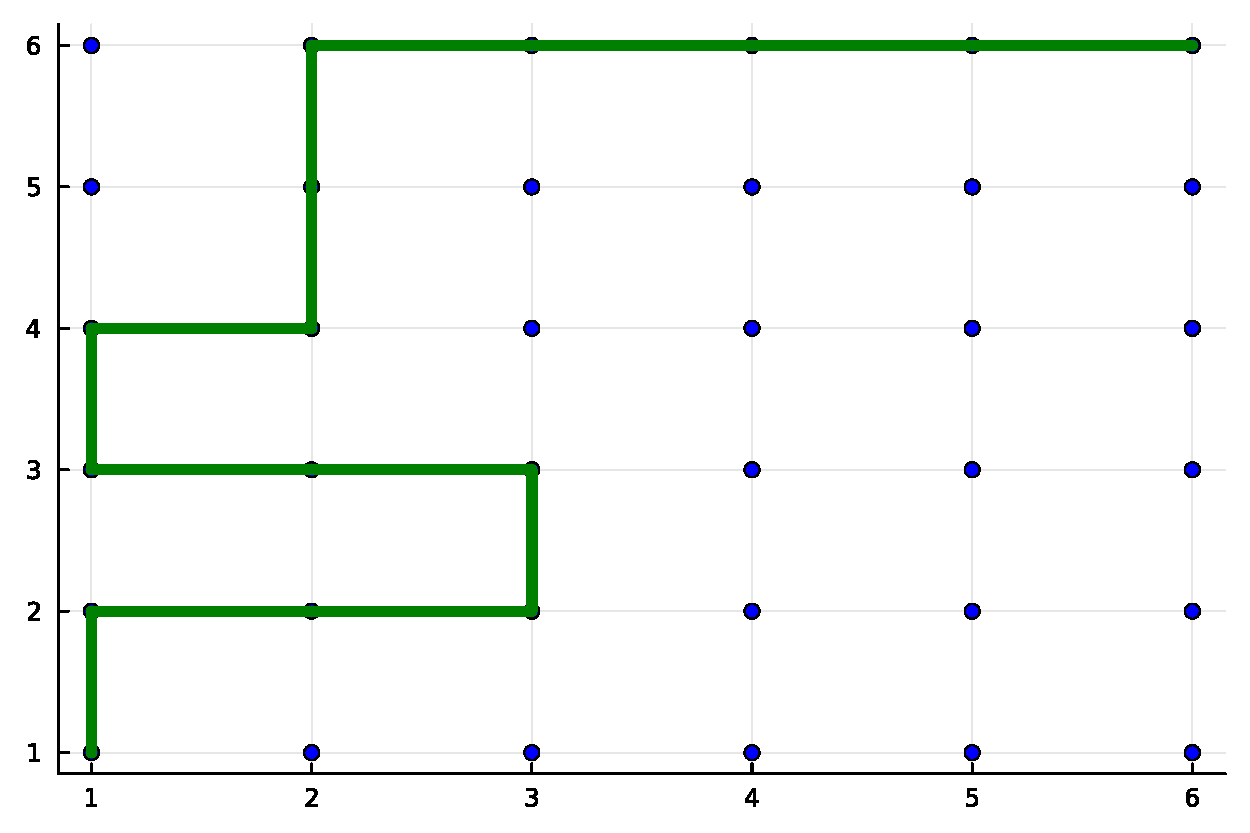
\includegraphics[scale=0.6]{images/movimento_tipo_linha.pdf}
    \caption{Deslocamento \emph{row-wise}.}
    \label{fig:exemplo movimento row-wise}
\end{figure}

\begin{figure}[ht]
    \centering
    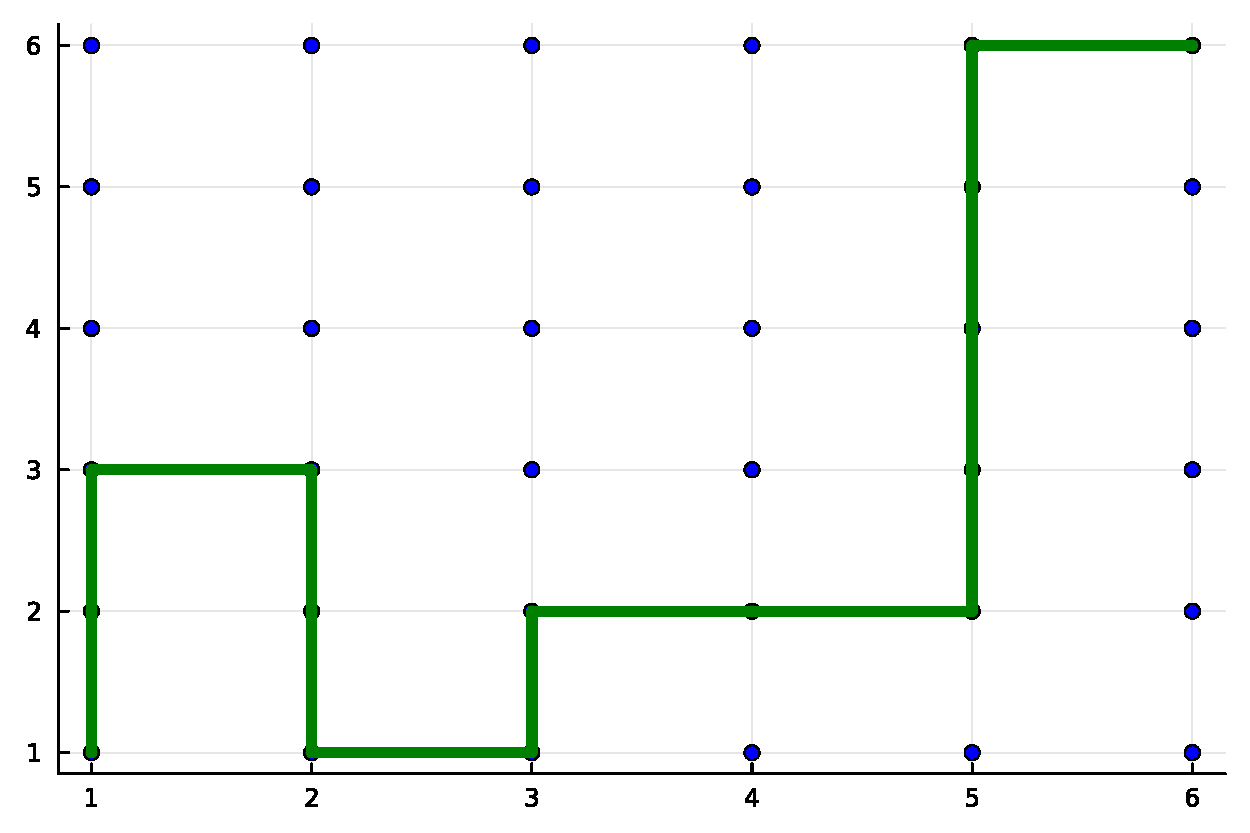
\includegraphics[scale=0.6]{images/movimento_tipo_coluna.pdf}
    \caption{Deslocamento \emph{column-wise}.}
    \label{fig:exemplo movimento column-wise}
\end{figure}

As \cref{fig:exemplo movimento row-wise,fig:exemplo movimento column-wise} assumem, implicitamente, que o movimento do robô segue um padrão de geometria táxi (ou Manhattan), em que o robô decompõe o percurso de menor distância até a próxima coordenada em trajetos puramente verticais e horizontais \cite{CESAR2010}. Os movimentos são assim definidos porque o deslocamento euclidiano equivalente pode resultar em colisões inesperadas com as quinas dos obstáculos retangulares. No entanto, existe uma questão a resolver: o robô deve fazer o movimento horizontal antes do vertical, ou o contrário? É para responder esta pergunta que a seção \emph{direction} (direção) existe no cromossomo. \emph{Direction} consiste em um vetor de $n - 1$ genes binários cujo $k$-ésimo gene descreve a ordem dos movimentos realizados do $k$-ésimo ponto de \emph{location} ao seu $(k+1)$-ésimo ponto. Nesta implementação, considera-se que o gene 0 indica que o movimento horizontal antecede o vertical, e o gene 1 indica o contrário.